\section{Frontend Model} 
The program's interface will be a website consisting of several web pages, including an index and login page, a worker page, and a customer page.

\subsection{Index and Login Page}
The login page should contain a simple form asking for a username and password. This page could also contain buttons to create a new user, and a button to change password.
\begin{figure}[H]
    \adjustbox{scale=0.6, center}{
        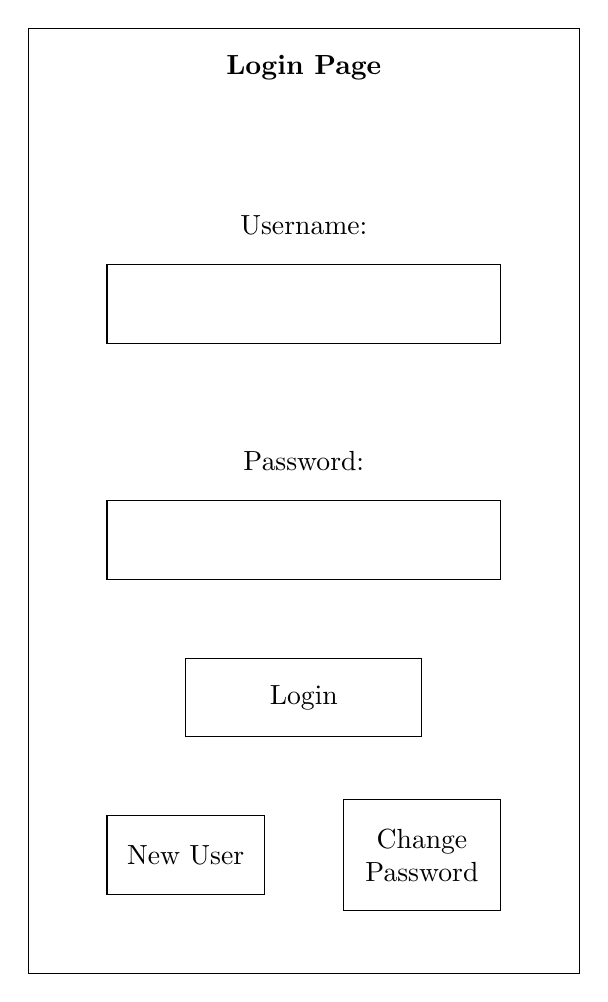
\begin{tikzpicture}
            \draw (0,0) rectangle (7,12);
        
            \draw[font=\bfseries] (3.5, 11.5) node {Login Page};
        
            \draw (3.5, 9.5) node {Username:};
            \draw (1,9) rectangle (6,8);
        
            \draw (3.5, 6.5) node {Password:};
            \draw (1,6) rectangle (6,5);
        
            \draw (2, 4) rectangle (5, 3);
            \draw (3.5, 3.5) node {Login};
        
            \draw (1,1) rectangle (3,2);
            \draw (2,1.5) node {New User};
            \draw (4,0.8) rectangle (6,2.2);
            \draw [align=center] (5, 1.5) node {Change\\Password};
        \end{tikzpicture}
    }
    \caption{An illustration of the login system.}
    \label{fig:LoginPage}
\end{figure}


\subsection{Worker Page}
The worker page should contain a button to toggle whether the worker node is doing work, as shown in Figure \ref{fig:WorkerPage}.

\begin{figure}[H]
    \adjustbox{scale=0.75, center}{
        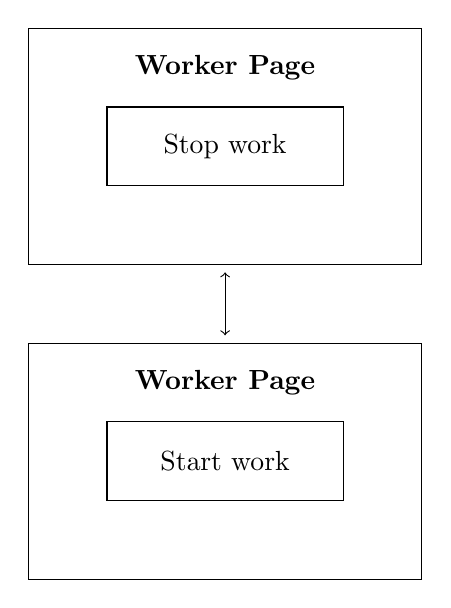
\begin{tikzpicture}
            \draw[font=\bfseries] (2.5,2.5) node {Worker Page};
            \draw(0,0) rectangle (5,3);
            \draw(1,1) rectangle (4,2);
            \draw (2.5, 1.5) node {Start work};
        
            \draw[<->] (2.5,3.1) -- (2.5,3.9);
        
            \draw[font=\bfseries] (2.5,6.5) node {Worker Page};
            \draw(0,4) rectangle (5,7);
            \draw(1,5) rectangle (4,6);
            \draw (2.5, 5.5) node {Stop work}; 
        \end{tikzpicture}
    }
    \caption{An illustration of the worker page.}
    \label{fig:WorkerPage}
\end{figure}


\subsection{Customer Page}
The customer page should interface with the master node. As shown in Figure \ref{fig:CustomerPage}, there should be a button for uploading files for processing, and a list of files ready to be downloaded.

\begin{figure}[H]
    \adjustbox{scale=0.75, center}{
        \usetikzlibrary{patterns}
        \begin{tikzpicture}
            \draw (0,0) rectangle (5,8);
        
            \draw (1,1.2) rectangle (4,1.8);
            \draw (2.5,1.5) node {thirdFile.csv};
        
            \draw (1,2.2) rectangle (4,2.8);
            \draw (2.5,2.5) node {secondFile.csv};
        
            \draw (1,3.2) rectangle (4,3.8);
            \draw (2.5,3.5) node {firstFile.csv};
        
            \draw (2.5, 4.5) node {Ready files download:};
        
            \draw(0.5, 5.5) rectangle (4.5, 5.8);
            \draw[pattern=north east lines](0.5, 5.5) rectangle (2, 5.8);
        
            \draw (1, 6) rectangle (4, 7);
            \draw (2.5,6.5) node {Upload file};
        \end{tikzpicture}
    }
    \caption{An illustration of the customer page.}
    \label{fig:CustomerPage}
\end{figure}